%iffalse
\let\negmedspace\undefined
\let\negthickspace\undefined
\documentclass[journal,12pt,onecolumn]{IEEEtran}
\usepackage{cite}
\usepackage{amsmath,amssymb,amsfonts,amsthm}
\usepackage{algorithmic}
\usepackage{graphicx}
\usepackage{textcomp}
\usepackage{xcolor}
\usepackage{txfonts}
\usepackage{listings}
\usepackage{enumitem}
\usepackage{enumitem,multicol}
\usepackage{mathtools}
\usepackage{gensymb}
\usepackage{comment}
\usepackage[breaklinks=true]{hyperref}
\usepackage{tkz-euclide} 
\usepackage{listings}
\usepackage{gvv}                                        
%\def\inputGnumericTable{}                                 
\usepackage[latin1]{inputenc}                                
\usepackage{color}                                            
\usepackage{array}                                            
\usepackage{longtable}                                       
\usepackage{calc}                                             
\usepackage{multirow}                                         
\usepackage{hhline}                                           
\usepackage{ifthen}                                           
\usepackage{lscape}
\usepackage{tabularx}
\usepackage{array}
\usepackage{float}
\usepackage[american,siunitx]{circuitikz}
\usetikzlibrary{arrows,shapes,calc,positioning}
\usepackage{pgfplots}


\newtheorem{theorem}{Theorem}[section]
\newtheorem{problem}{Problem}
\newtheorem{proposition}{Proposition}[section]
\newtheorem{lemma}{Lemma}[section]
\newtheorem{corollary}[theorem]{Corollary}
\newtheorem{example}{Example}[section]
\newtheorem{definition}[problem]{Definition}
\newcommand{\BEQA}{\begin{eqnarray}}
\newcommand{\EEQA}{\end{eqnarray}}
\newcommand{\define}{\stackrel{\triangle}{=}}
\theoremstyle{remark}
\newtheorem{rem}{Remark}

% Marks the beginning of the document
\begin{document}
\bibliographystyle{IEEEtran}
\vspace{3cm}

\title{XE-2016}
\author{EE24Btech11022 - Eshan Sharma}
\maketitle

\renewcommand{\thefigure}{\theenumi}
\renewcommand{\thetable}{\theenumi}



\begin{enumerate}
\item The flow field shown over a bluff body has considerably curved streamlines. A student measures pressures at points $A$, $B$, $C$, and $D$ and denotes them as $P_A$, $P_B$, $P_C$, and $P_D$ respectively. State which one of the following statements is true. The arrow indicates the freestream flow direction.\\

\begin{center}
	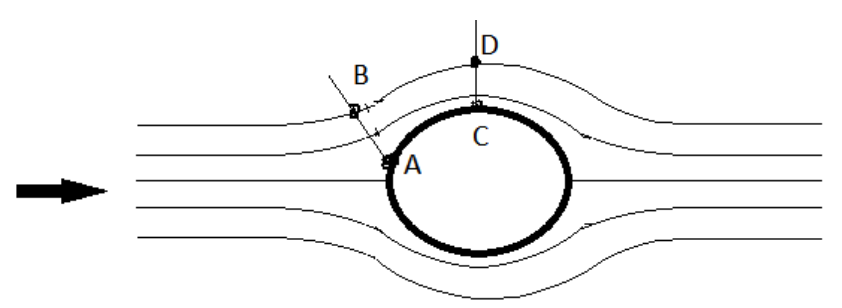
\includegraphics[width=0.6\textwidth]{figs/27.png}
\end{center}

\begin{enumerate}
	\item $P_A = P_B$ and $P_C > P_D$
	\item $P_A > P_B$ and $P_C > P_D$
	\item $P_A = P_B$ and $P_C < P_D$
	\item $P_A > P_B$ and $P_C < P_D$\\
\end{enumerate}

\item A 2-D incompressible flow is defined by its velocity components in m/s as $u = -\frac{c y}{x^2 + y^2}$ and $v = \frac{cx}{x^2 + y^2}$. If the value of the constant $c$ is equal to 0.1 m\(^3\), the numerical value of vorticity at the point $x = 1$ m and $y = 2$ m is \_\_\_\_\_ s\(^{-1}\).\\

\item Two flow configurations are shown below for flow of incompressible, viscous flow. The inlet velocity for the diverging nozzle (Fig (i)) and free-stream velocity for flow past the bluff body (Fig (ii)) is constant. Points $A$ and $B$ are separation points and flow is laminar. The relation regarding velocity gradients at point $A$ and $B$ is ($y$ is the direction normal to the surface at the point of separation).\\

\begin{center}
	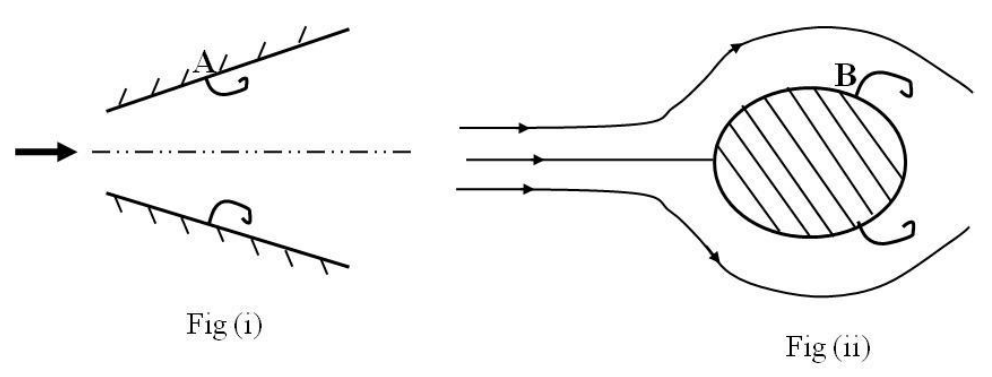
\includegraphics[width=0.8\textwidth]{figs/29.png}
\end{center}

\begin{enumerate}
\begin{multicols}{4}
	\item $\frac{\partial u}{\partial y}\bigg|_A = \frac{\partial u}{\partial y}\bigg|_B$
	\item $\frac{\partial u}{\partial y}\bigg|_A > \frac{\partial u}{\partial y}\bigg|_B$
	\item $\frac{\partial u}{\partial y}\bigg|_A < \frac{\partial u}{\partial y}\bigg|_B$
	\item $\frac{\partial^{2} u}{\partial y^{2}}\bigg|_A = \frac{\partial^{2} u}{\partial y^{2}}\bigg|_B$
\end{multicols}
\end{enumerate}

\item Consider a fully developed, steady, incompressible, 2-D, viscous channel flow with uniform suction and blowing velocity $v_0$ as shown in the figure below. The centerline velocity of the channel is 10 m/s along the $x$-direction. If the value of $v_0$ at both the walls is 1 m/s, the value of the $y$-component of velocity inside the flow field is \_\_\_\_\_ m/s.\\

\begin{center}
	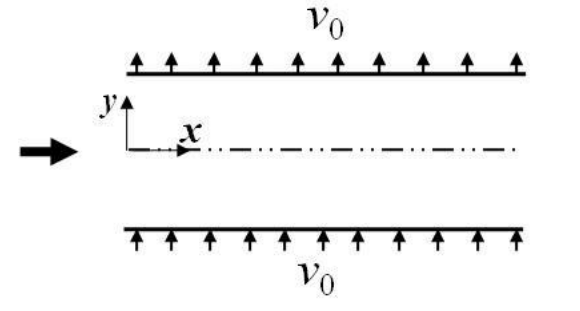
\includegraphics[width=0.6\textwidth]{figs/30.png}
\end{center}


\item Exhaust from a kitchen goes into the atmosphere through a tapered chimney as shown. The area of cross-section of a chimney at location-1 is twice of that at location-2. The flow rate is assumed to be steady with constant exhaust density of 1 kg/m$^3$ and acceleration due to gravity, $g = 9.8$ m/s$^2$. If the steady uniform exhaust velocity at location-1 is $U = 1$ m/s, the pressure drop across the chimney is \_\_\_\_ Pa.\\

\begin{center}
	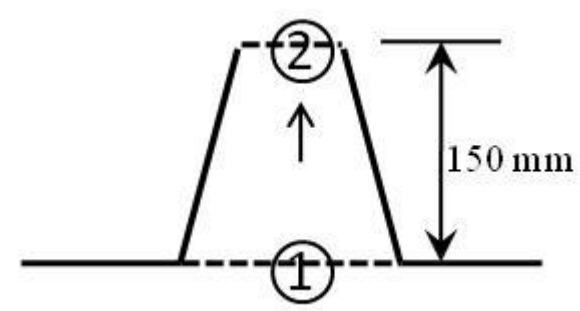
\includegraphics[width=0.6\textwidth]{figs/31.png}
\end{center}

\item A jet of diameter 20 mm and velocity 6 m/s coming out of a water-tank standing on a frictionless cart hits a vane and gets deflected at an angle of 45\degree\ as shown in the figure below. The density of water is 1000 kg/m$^3$. Neglect all minor and viscous losses. If the cart remains stationary, the magnitude of tension in the supporting string connected to the wall is \_\_\_\_ N.\\

\begin{center}
	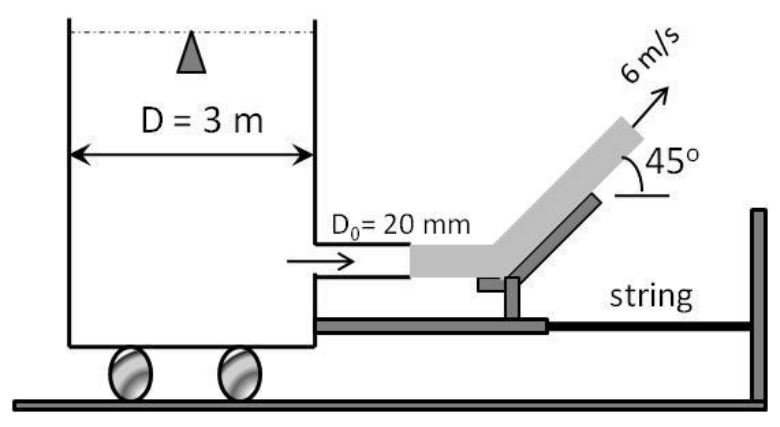
\includegraphics[width=0.6\textwidth]{figs/32.png}
\end{center}

\item A block is floating at the oil-water interface as shown. The density of oil is two-thirds that of water. Given that the density of the block is 800 kg/m$^3$ and that of water is 1000 kg/m$^3$, the fraction of the total height of block in oil is \_\_\_\_.\\

\begin{center}
	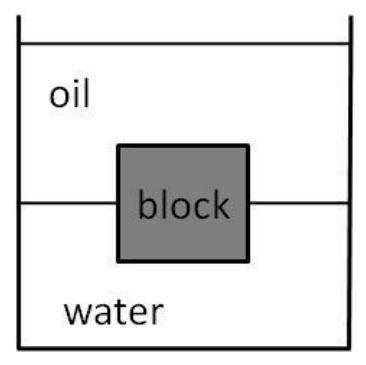
\includegraphics[width=0.3\textwidth]{figs/33.png}
\end{center}

\item A horizontal pipe is feeding water into a reservoir from the top with a time-dependent volumetric flow rate, $\vec{Q}\brak{m^{3}/h} = 1+0.1 \times t$, where $t$ is in hours. The area of the base of the reservoir is $0.5 m^2$. Assuming that initially the reservoir is empty, the height of the water level in the reservoir after 60 minutes is \_\_\_\_ m.\\

\item Velocity field of a 2-D steady flow is provided as $\vec{V} = c\brak{x^2-y^2}\hat{i} - 2cxy\hat{j}$. The equation of streamlines of this flow is:

\begin{enumerate}
\begin{multicols}{2}
	\item $x^2y - \frac{y^2}{3} = \text{Constant}$
	\item $xy^2 - \frac{y^2}{3} = \text{Constant}$
	\item $xy - \frac{y}{3} = \text{Constant}$
	\item $x^2y - \frac{y^3}{3} = \text{Constant}$
\end{multicols}
\end{enumerate}

\item Velocity potential and stream function in polar coordinates $(r, \theta)$ for a potential flow over a cylinder with radius $R$ is given as $\phi = U_\infty \left(r + \frac{R^2}{r}\right)\cos\theta$ and $\psi = U_\infty \left(r - \frac{R^2}{r}\right)\sin\theta$, respectively. Here, $U_\infty$ denotes uniform freestream velocity, and $\theta$ is measured counter clockwise as shown in the figure. How does the velocity magnitude, $\vec{q}$, over the surface of the cylinder will vary?

\begin{center}
	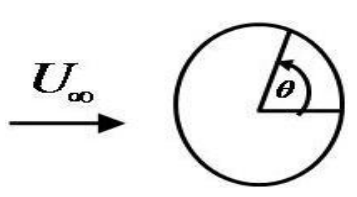
\includegraphics[width=0.6\textwidth]{figs/36.png}
\end{center}

\begin{enumerate}
\begin{multicols}{2}
	\item $\vec{q} = 2U_\infty \cos\theta$
	\item $\vec{q} = U_\infty \cos2\theta$
	\item $\vec{q} = 2U_\infty \sin2\theta$
	\item $\vec{q} = 2U_\infty \sin\theta$
\end{multicols}
\end{enumerate}

\item Consider a laminar flow of water over a flat plate of length $L = 1$ m. The boundary layer thickness at the end of the plate is $\delta_w$ for water, and $\delta_a$ for air for the same freestream velocity. If the kinematic viscosities of water and air are $1 \times 10^{-6}$ m$^2$/s and $1.6 \times 10^{-5}$ m$^2$/s, respectively, the numerical value of the ratio $\frac{\delta_w}{\delta_a}$ is \_\_\_\_.\\


\item Prototype of a dam spillway (a structure used for controlled release of water from the dam) has characteristic length of 20 m and characteristic velocity of 2 m/s. A small model is constructed by keeping Froude number same for dynamic similarity between the prototype and the model. What is the minimum length-scale ratio between prototype and the model such that the minimum Reynolds' number for the model is 100? The density of water is 1000 kg/m$^3$ and viscosity is $10^{-3}$ Pa$\cdot$s.

\begin{multicols}{4}
	\begin{enumerate}
		\item $1.8 \times 10^{-4}$
		\item $1 \times 10^{-4}$
		\item $1.8 \times 10^{-3}$
		\item $9.1 \times 10^{-4}$
	\end{enumerate}
\end{multicols}

\item An orifice meter, having orifice diameter of $d = \frac{20}{\sqrt{\pi}}$ mm, is placed in a water pipeline having flow rate, $Q_{\text{act}} = 3 \times 10^{-4}$ m$^3$/s. The ratio of orifice diameter to pipe diameter is 0.6. The contraction coefficient is also 0.6. The density of water is 1000 kg/m$^3$. If the pressure drop across the orifice plate is 43.5 kPa, the discharge coefficient of the orifice meter at this flow Reynolds number is \_\_\_\_\_\_\_.

\end{enumerate}
\end{document}


